% !TEX root = OptimalOffline.tex

We now proceed to relax the condition that the receiver harvests energy only once. The receiever harvests energy equivalent to the amount required to stay on for time $\TRx_i$ at time instances $r_i$. 
We assume that the receiver has an infinite battery capacity. 
Again, since we are considering the offline case, we assume we have knowledge of the receiver energy arrivals non causally. This can be stated as an optimization problem as follows.\\
\begin{problem}
\begin{align}
&\min_{\{\textbf{p},\textbf{s},N\}}			&& T
\\
&\text{subject to} 				&& B(T)=B_0, 
\label{pb2_constraint_bits}
\\
&     										&& U(t)\le \mathcal{E}(t)  		\;\;\;\;\;\; \forall \; t\;\in\;[0,T], \label{pb2_constraint_energy}
\\
&    										&& \displaystyle \sum_{i=1}^k \mathcal{S}_i(s_{i+1} - s_i) + \mathcal{S}_i(t - s_{k+1}) \leq \TRx(t) \\ &&&\forall \; t \; in \; [0,T] \; \text{where} \; k = \max\{i| s_{i+1} \leq t\}.
\label{pb2_constraint_time}
\end{align}
\end{problem}
$\mathcal{S}_i:\mathbb{Z}\rightarrow\{0,1\}$ is a function that takes value $1$ if $p_i>0$ and $0$ otherwise.\\
Our approach to solve this problem will be to use the previously derived algorithm and try to apply it iteratively. Let $O_i$ be the first time instance such that if the receiver is started for the first time at $O_i$ and kept on continuously, then it will be able to stay on for $\TRx(r_i)$ time. It can be easily shown, (and seen in figure \ref{figure_origin_points}) that the receiver will exhaust all its energy at at least one energy arrival epoch $r_m$ when it transmits from $O_i$ for $\TRx(r_i)$ time. For example, in the figure, when the receiver transmits starting from $O_1$, it exhausts all it's energy at $r_1^-$. Since the reciever uses a constant amount of power, $O_i = r_m - \TRx(r_{m-1})$. This can be visualised in figure \ref{figure_origin_points}. Now, we prove the following lemmas.\\

\begin{figure}
\centering
  \centerline{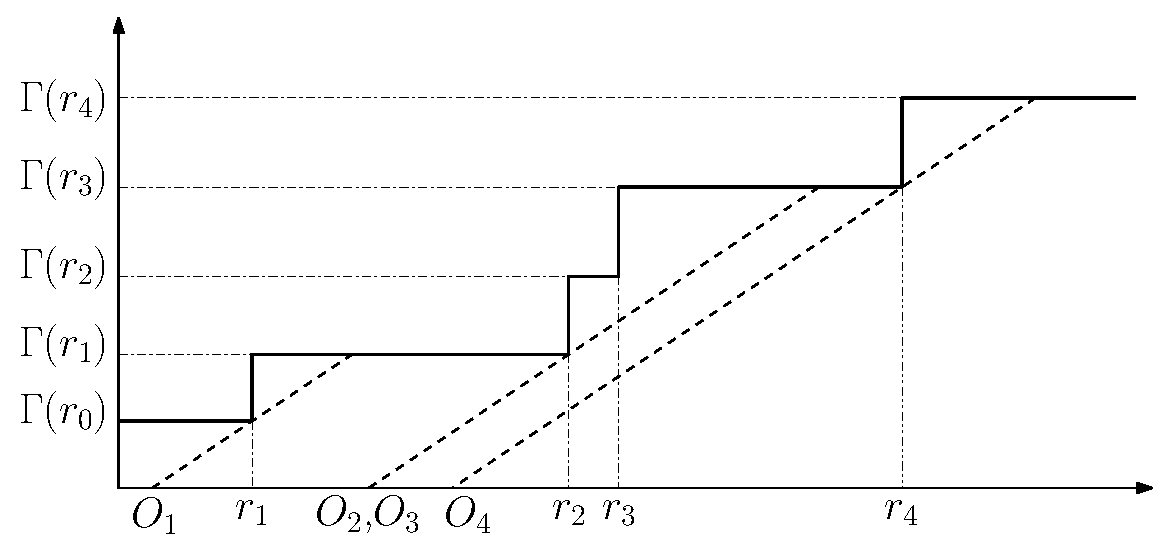
\includegraphics[width=8cm]{origin_points.eps}}
\caption{Figure showing $O_i$'s which represent the first time instances at which the reciever can be kept on continuously for $\TRx(r_i)$ time. Note that $O_2$ and $O_3$ coincide in this example.}\label{figure_origin_points}
\end{figure}

\begin{lemma}
If a policy $\{\bm{p},\bm{s},N\}$ for Problem 2 is optimal, either $s_1 = O_i$ for some $i$, and/or the receiver remains on for exactly $\TRx(r_i)$ time for some $i$.
\label{lemma_startpoints}
\end{lemma}

\begin{lemma}
A solution $\{\bm{p},\bm{s},N\}$, arrived at by passing $O_i$ and $\TRx(r_t)$ into Algorithm 1 can only be optimal if $O_i\leq s_1\leq O_{i+1}$.
\label{lemma_startpoints}
\end{lemma}

\begin{table}
\begin{minipage}[b]{8cm}
\caption {Offline algorithm for energy arrival in receiver after time t=0}
\begin{tabular}{p{7cm}}
\hline \textbf{Input}: Bits to transmit $B_0$; $\ETx_i$, $\TRx_i$ for all $i$
\\
\hline
\\
\textbf{Initialize:}
\\ 
$u=\min u_i$ s.t. $\TRx(u_i)g\left( \dfrac{\ETx(u_i)}{\TRx(u_i)} \right) \ge B_0$. $O_f=\infty$.\\ $u_1=min(r_1,t_1),u_2=min(..)$
\\
For all $i$, define $O_i=\min$ $t$ s.t. receiver can be \textit{on} from $t$ to $(t+\TRx(r_i))$, i.e. $x-t \le \TRx(x)$,  $t \le x\le (t+\TRx(r_i))$.
\\
\\
\textbf{if} $u=r_j$ for some $j$  \textbf{then}
\\
\hspace{4mm}$O_l=O_{j}$, $T=\TRx(r_j)$
\\
\textbf{else}
\\
\hspace{4mm}Let $u=t_j$ for some $j$
\\
\hspace{4mm}$u_{j'}=\min r_i$ s.t. $\TRx(r_i)g\Bigg{(} \dfrac{\ETx(t_j)}{\TRx(r_i)}\Bigg{)}\ge B_0$
\\
\hspace{4mm}$O_l=O_{j'}$, $T=\TRx(r_{j'})$.
\\
\textbf{end if}
\\
\textbf{do}
\\
\hspace{4mm}Apply $Algo1(O_l,T)\rightarrow T_{opt}$
\\
\hspace{4mm}$r_k=\max_i r_i $ s.t. $r_i<T_{opt}$ 
\\
\hspace{4mm}\textbf{if} $O_{f} > O_{k}$
\\
\hspace{7mm}$O_{f} = O_{k}$
\\
\hspace{4mm}\textbf{end if}
\\
\hspace{4mm}\textbf{if} hit origin \textbf{then} $l=l-1$ \textbf{else} $l=l+1$
\\
\textbf{while} $O_l \le O_{f}$
\\
\hline
\label{online}
\end{tabular}
\end{minipage}
\end{table}
